\chapter{The CMS experiment at the \LHC}
\label{chap:detector}

% \chapterquote{There, sir! that is the perfection of vessels!}
% {Jules Verne, 1828--1905}

\section{The \LHC}
\label{sec:lhc}

% \begin{figure}
%   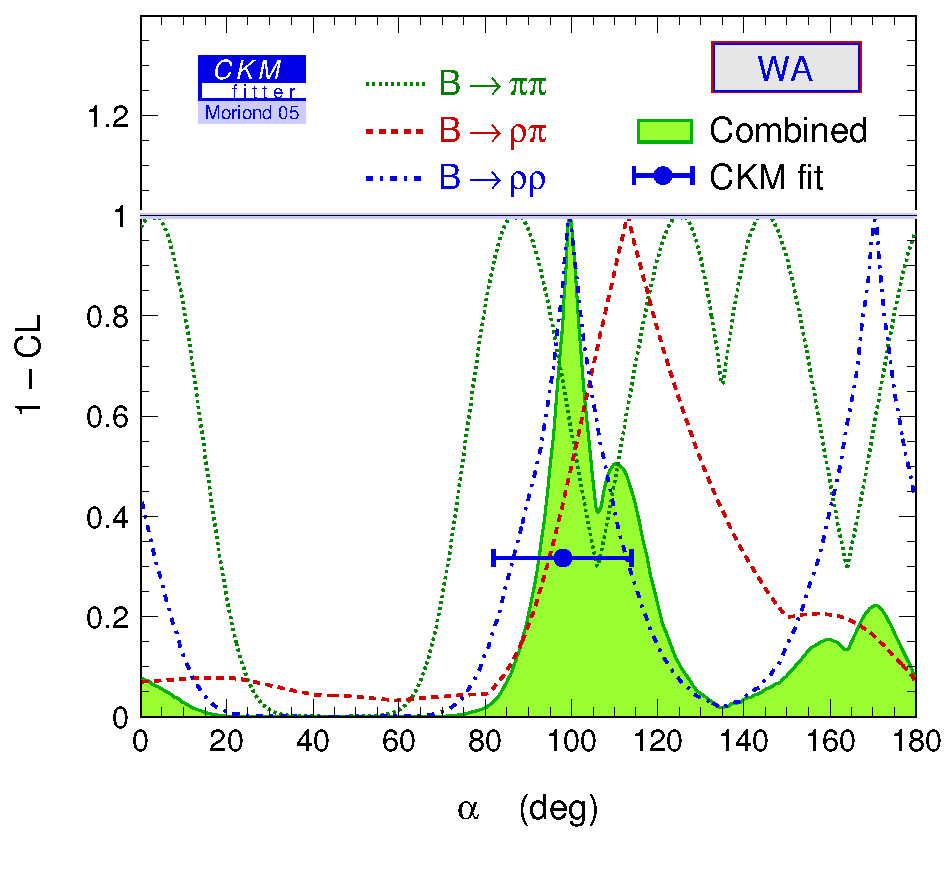
\includegraphics[width=\largefigwidth]{ckmfitter-alpha-combined}
%   \caption[CKM Fitter constraints on \alphaCKM.]%
%   {CKM Fitter constraints on \alphaCKM from combined \BToPiPi,
%     \BToRhoPi and \BToRhoRho decay analyses.}
%   \label{fig:CKMFitter}
% \end{figure}

\section{The CMS detector}
\label{sec:cms}

\subsection{Trigger system}
\label{sec:triggers}

% \begin{table}[bp]
%   \begin{tabular}{lllll}
%                 & L0              & L1              & HLT             \\
%     \midrule\\
%     Input rate  & \unit{40}{\MHz} & \unit{1}{\MHz}  & \unit{40}{\kHz} \\
%     Output rate & \unit{1}{\MHz}  & \unit{40}{\kHz} & \unit{2}{\kHz}  \\
%     Location    & On detector     & Counting room   & Counting room   \\
%   \end{tabular}
%   \caption{Characteristics of the trigger levels and offline analysis.}
%   \label{tab:TriggerDetails}
% \end{table}
